% SC4242 --- Chapter 5: IR 3AC and SSA (0->100 ground-up)
\chapter{Intermediate Representations: 3AC and SSA}
\label{ch:ir}

\begin{quote}
\emph{``A good IR is half the compiler.''} --- Between AST and assembly, a uniform, low-level yet machine-independent IR lets one optimiser serve many languages and targets.
\end{quote}

\noindent\fbox{\parbox{\dimexpr\linewidth-2\fboxsep-2\fboxrule}{%
\textbf{From zero: we build here, no IR assumed.} We define three-address code, basic blocks, control-flow graphs, dominance, and static single assignment from sets and graphs. Every transformation is shown on a running example: factorial.}}
\vspace{0.4em}

\section*{Learning Outcomes}
After this chapter you will be able to:
\begin{enumerate}[label=(L\arabic*)]
    \item lower AST expressions/statements to three-address code with temporaries and labels;
    \item partition 3AC into basic blocks and build the control-flow graph (CFG);
    \item define dominance, immediate dominance, dominator tree, and dominance frontier;
    \item convert a CFG to SSA form via $\phi$-placement (Cytron) and renaming;
    \item explain mem2reg, SSA destruction, and why SSA simplifies optimisation.
\end{enumerate}

% ============================================================
\section{Three-Address Code}
\label{sec:3ac}
\emph{Intuition:} an AST nests arbitrarily; 3AC flattens to ``at most one operation per line'' with explicit temporaries---like assembly without registers.

\begin{definition}[3AC]
Instructions: $x \gets y\ \text{op}\ z$ (binary), $x\gets\text{op }y$ (unary), $x\gets y$ (copy), $\texttt{goto }L$, $\texttt{if }x\ \text{relop}\ y\texttt{ goto }L$, $x\gets y[z]$ / $x[z]\gets y$ (array), $x\gets\texttt{call }f(args)$, $\texttt{return }x$, $\texttt{label }L$. Each has $\le3$ addresses (hence the name). Temporaries $t_1,t_2,\dots$ hold intermediate results.
\end{definition}

\begin{example}[Lowering expression]
AST \texttt{a = b + c*2} $\to$ 3AC:
\begin{lstlisting}[language=C]
t1 = c * 2
t2 = b + t1
a  = t2
\end{lstlisting}
If source had \texttt{if (x < 10) y=1 else y=2}, we emit conditional branches and labels (next section). Short-circuit \texttt{a \&\& b} lowers to branching, not bitwise \texttt{and}.
\end{example}

Lowering walks the AST, threading a fresh-temp counter and a label generator. For boolean contexts, we use \emph{jumping code}: \texttt{E} in condition position emits jumps to true/false labels instead of a boolean value.

% TikZ 1: AST -> 3AC -> CFG flow
\begin{figure}[h]
\centering
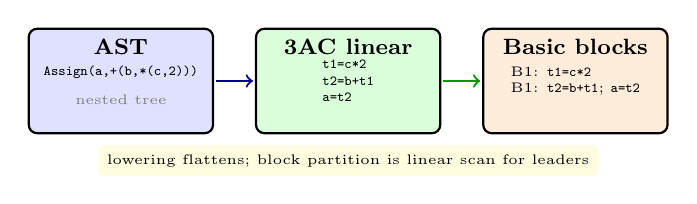
\begin{tikzpicture}[scale=0.78,every node/.style={font=\scriptsize}]
\draw[thick,fill=blue!12,rounded corners=3pt] (0,0) rectangle (3.0,1.7);
\node[font=\footnotesize\bfseries] at (1.5,1.4) {AST};
\node[font=\tiny] at (1.5,1.0) {\texttt{Assign(a,+(b,*(c,2)))}};
\node[font=\tiny,gray] at (1.5,0.55) {nested tree};
\draw[->,thick,blue!60!black] (3.05,0.85)--(3.65,0.85);
\draw[thick,fill=green!14,rounded corners=3pt] (3.7,0) rectangle (6.7,1.7);
\node[font=\footnotesize\bfseries] at (5.2,1.4) {3AC linear};
\node[font=\tiny,align=left] at (5.2,0.85) {\texttt{t1=c*2}\\ \texttt{t2=b+t1}\\ \texttt{a=t2}};
\draw[->,thick,green!60!black] (6.75,0.85)--(7.35,0.85);
\draw[thick,fill=orange!14,rounded corners=3pt] (7.4,0) rectangle (10.4,1.7);
\node[font=\footnotesize\bfseries] at (8.9,1.4) {Basic blocks};
\node[font=\tiny,align=left] at (8.9,0.85) {B1: \texttt{t1=c*2}\\ B1: \texttt{t2=b+t1}; \texttt{a=t2}};
\node[font=\tiny,fill=yellow!12,rounded corners=2pt] at (5.2,-0.45) {lowering flattens; block partition is linear scan for leaders};
\end{tikzpicture}
\caption{Lowering AST to linear 3AC then partitioning into basic blocks. Leaders are first instruction, jump targets, and instructions after jumps.}
\label{fig:ast-to-cfg}
\end{figure}

% ============================================================
\section{Basic Blocks and CFGs}
\label{sec:cfg}
A \emph{basic block} is a maximal straight-line sequence with one entry (first instr) and one exit (last instr, a jump/branch/return). Partition by marking \emph{leaders}: (i) first instruction, (ii) any label target, (iii) instruction after a jump. Blocks become CFG nodes; edges are ``may jump to''.

\begin{example}[Factorial CFG]
Source \texttt{fact(n) \{ r=1; while(n>1)\{r=r*n; n=n-1\} return r\}} gives blocks: B1 \texttt{r=1}, B2 header \texttt{if n>1 goto B3 else B5}, B3 body \texttt{r=r*n; n=n-1; goto B2}, B5 \texttt{return r}. Edges B1$\to$B2, B2$\to$B3/B5, B3$\to$B2. See Fig.~\ref{fig:cfg-fact}.
\end{example}

% TikZ 2: factorial CFG before SSA + dominator tree
\begin{figure}[h]
\centering
\begin{tikzpicture}[>=Stealth,scale=0.78,every node/.style={font=\scriptsize}]
% CFG
\begin{scope}
\draw[thick,fill=blue!10,rounded corners=3pt] (0,2.0) rectangle (3.0,2.7);
\node[font=\footnotesize\bfseries] at (1.5,2.85) {CFG};
\node[draw,fill=blue!12,rounded corners=3pt] (b1) at (1.5,2.35) {B1: r=1};
\node[draw,fill=green!14,rounded corners=3pt] (b2) at (1.5,1.55) {B2: if n>1 ?};
\node[draw,fill=orange!14,rounded corners=3pt] (b3) at (0.3,0.65) {B3: r*=n; n-- };
\node[draw,fill=violet!12,rounded corners=3pt] (b5) at (2.7,0.65) {B5: return r};
\draw[->,thick,blue!60!black] (b1)--(b2);
\draw[->,thick,green!60!black] (b2)--(b3) node[midway,left,font=\tiny] {T};
\draw[->,thick,green!60!black] (b2)--(b5) node[midway,right,font=\tiny] {F};
\draw[->,thick,orange!60!black] (b3) to[bend left=22] (b2);
\end{scope}
% dominator tree
\begin{scope}[xshift=5.2cm]
\draw[thick,fill=blue!10,rounded corners=3pt] (0,2.0) rectangle (5.2,2.7);
\node[font=\footnotesize\bfseries] at (2.6,2.85) {Dominator tree};
\node[draw,circle,fill=blue!16] (d1) at (2.6,2.35) {B1};
\node[draw,circle,fill=green!14] (d2) at (2.6,1.55) {B2};
\node[draw,circle,fill=orange!14] (d3) at (1.2,0.65) {B3};
\node[draw,circle,fill=violet!12] (d5) at (4.0,0.65) {B5};
\draw[->,thick,blue!60!black] (d1)--(d2);
\draw[->,thick,green!60!black] (d2)--(d3);
\draw[->,thick,green!60!black] (d2)--(d5);
\node[font=\tiny,fill=yellow!12,rounded corners=2pt] at (2.6,0.05) {idom(B3)=B2, idom(B5)=B2};
\end{scope}
\end{tikzpicture}
\caption{Factorial CFG (left) and its dominator tree (right). B1 dominates all; B2 dominates loop body and exit. Dominance frontier of B3 is \{B2\}---where $\phi$ for loop-carried \texttt{r,n} will appear.}
\label{fig:cfg-fact}
\end{figure}

% ============================================================
\section{Dominance and SSA}
\label{sec:ssa}
\emph{Intuition:} in straight-line code, each variable has one value reaching each use. Branches and loops merge values. SSA makes the merge explicit with $\phi$-functions: ``this variable is whichever predecessor's value arrived''.

\begin{definition}[Dominance]
Node $d$ \emph{dominates} $n$ ($d\ \mathbf{dom}\ n$) if every path entry$\to n$ includes $d$. \emph{Strict}, \emph{immediate dominator} \texttt{idom} (closest strict dominator), and \emph{dominator tree} (idom edges) follow. The \emph{dominance frontier} $\text{DF}(n)=\{y\mid n\text{ doms a pred of }y\text{ but not }y\text{ strictly}\}$---exactly where $\phi$ may be needed.
\end{definition}
Dominator tree via Lengauer--Tarjan $O((V+E)\log(V+E))$; $\text{DF}$ by walking.

\begin{definition}[SSA]
Each variable assigned exactly once. Multiple assignments become versions $x_1,x_2,\dots$; at control merges, $x_3\gets\phi(x_1,x_2)$ selects the incoming value. Fig.~\ref{fig:ssa-fact} shows factorial after SSA: \texttt{r1} before loop, \texttt{r2=$\phi$(r1,r3)} at header, similarly \texttt{n2=$\phi$(n1,n3)}.
\end{definition}

\begin{example}[Why $\phi$ lives at DF]
Consider diamond $A\texttt{: }x=1 \to B,C \to D\texttt{: }y=x$. $A$ dominates $B,C$ but not $D$ strictly (both $B,C$ reach $D$). The merge at $D$ is exactly the frontier of $\{B,C\}$ (where definitions from one side stop dominating the join). Inserting $\phi(x)$ at $D$ makes $y$'s use see the correct incoming version without searching predecessors.
\end{example}

% TikZ 3: SSA form of factorial
\begin{figure}[h]
\centering
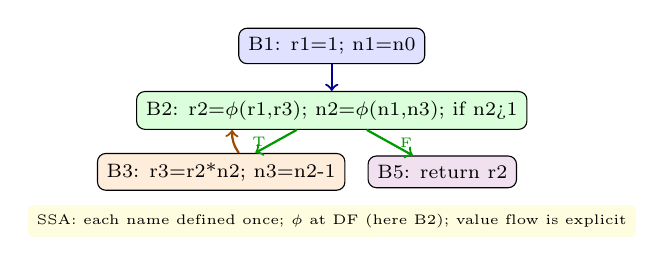
\begin{tikzpicture}[scale=0.78,every node/.style={font=\scriptsize}]
\node[draw,fill=blue!12,rounded corners=3pt] (b1) at (2.0,2.4) {B1: r1=1; n1=n0};
\node[draw,fill=green!14,rounded corners=3pt] (b2) at (2.0,1.35) {B2: r2=$\phi$(r1,r3); n2=$\phi$(n1,n3); if n2>1};
\node[draw,fill=orange!14,rounded corners=3pt] (b3) at (0.2,0.35) {B3: r3=r2*n2; n3=n2-1};
\node[draw,fill=violet!12,rounded corners=3pt] (b5) at (3.8,0.35) {B5: return r2};
\draw[->,thick,blue!60!black] (b1)--(b2);
\draw[->,thick,green!60!black] (b2)--(b3) node[midway,left,font=\tiny] {T};
\draw[->,thick,green!60!black] (b2)--(b5) node[midway,right,font=\tiny] {F};
\draw[->,thick,orange!60!black] (b3) to[bend left=18] (b2);
\node[font=\tiny,fill=yellow!12,rounded corners=2pt] at (2.0,-0.45) {SSA: each name defined once; $\phi$ at DF (here B2); value flow is explicit};
\end{tikzpicture}
\caption{Factorial in SSA. Cytron placement inserts $\phi$ for \texttt{r,n} at DF of their definitions (B2); renaming then versions them. Optimisations now see defs dominate uses.}
\label{fig:ssa-fact}
\end{figure}

\paragraph{Cytron SSA construction.}
1) Insert $\phi$: for each variable $x$, let $Defs=\{blocks\ defining\ x\}$; iterated $\text{DF}^+$ (worklist adding $\text{DF}$ of newly inserted) places $\phi$ for $x$ at each frontier block. 2) Rename: DFS over dominator tree, maintaining version stacks per variable; on defining instruction assign fresh version and push; on use replace with stack top; on $\phi$ define new version; pop on exit. Complexity near-linear.

\begin{lstlisting}[language=Python]
def ssa_rename(block, stacks, counter):
    # stacks[x] = list of current versions; counter[x] = next fresh id
    for phi in block.phis:                 # e.g. r2 = phi(r1,r3)
        v = new_version(phi.var, counter); stacks[phi.var].append(v); phi.dst=v
    for inst in block.insts:
        for i, use in enumerate(inst.uses): inst.uses[i]=stacks[use.var][-1]
        if inst.defs:
            v = new_version(inst.def.var, counter)
            stacks[inst.def.var].append(v); inst.def=v
    for succ in block.succs:               # fix phi operands
        for phi in succ.phis:
            if phi.var in stacks: phi.args[block.id]=stacks[phi.var][-1]
    for child in dom_tree[block.id]: ssa_rename(child, stacks, counter)
    for phi in block.phis: stacks[phi.var].pop()
    for inst in block.insts:
        if inst.defs: stacks[inst.def.orig].pop()
\end{lstlisting}

\paragraph{Why SSA helps.} Def-use chains are explicit; dominance $\Rightarrow$ cheap liveness; many optimisations become sparse. Destruction (out of SSA) replaces $\phi$ by copies on predecessor edges, coalescing to reduce moves.

\paragraph{From 3AC to SSA to target (mem2reg).}
Source variables may be \emph{memory} (stack slots) initially: \texttt{alloca} + \texttt{load}/\texttt{store}. The \emph{mem2reg} promotion identifies allocas whose address never escapes and whose loads/stores are analysed as above; those become SSA registers, phi-inserted exactly as for \texttt{r,n}. This is often the first optimisation pass: after it, dataflow is sparse. LLVM's \texttt{-mem2reg} does this; GIMPLE's ``out of SSA'' must respect calling convention copies.

\paragraph{IR design choices.}
How high-level should IR be? LLVM IR keeps types and typed pointers for alias analysis; some IRs are untyped but add explicit bounds checks. Multi-level IR (MLIR) stacks dialects: high-level loops $\to$ affine $\to$ CFG $\to$ machine. The principle: keep IR that makes the next analysis easy, not that mirrors source syntax. That is why AST $\to$ 3AC $\to$ SSA is the canonical lowering pipeline.

\paragraph{Critical edges and splitting.}
An edge $u\to v$ is \emph{critical} if $u$ has $\ge2$ successors and $v$ has $\ge2$ predecessors. $\phi$-copy insertion or code motion on such edges needs a new block (edge splitting) to hold the inserted code without affecting other paths. Compilers split critical edges before SSA destruction and before many loop opts; the CFG shape after splitting has no critical edges, simplifying correctness proofs.

\begin{example}[3AC with labels for factorial]
\begin{lstlisting}[language=C]
L1: r=1
L2: if n>1 goto L3 else L5
L3: r=r*n; n=n-1; goto L2
L5: return r
\end{lstlisting}
Leaders are \texttt{L1,L2,L3,L5}; blocks are maximal sequences between leaders. The CFG edges are exactly the \texttt{goto}/\texttt{if-goto} targets plus fall-through. This labelled view is what the partition pass emits before building CFG successor lists.
\end{example}

% ============================================================
\section{Chapter Notes}
3AC is due to UNCOL dreams; LLVM IR and GCC GIMPLE are modern instances. SSA was invented by Rosen--Wegner--Zadeck (1988) and normalised by Cytron et al.\ (1991). Dominance via Lengauer--Tarjan (1979) remains the fastest. For practice, ``SSA book'' (Boissinot et al.) and Appel/Lattner give construction details; mem2reg (promoting stack slots to SSA) is often a student's first pass.

% ============================================================
\section{Exercises}
\label{sec:ch05-exercises}
\begin{enumerate}[label=E5.\arabic*, leftmargin=*, itemsep=0.8em]
\item \textbf{Lower + partition.} Lower \texttt{while(x<10)\{ if(y>0) x=x+1 else x=x+2\}} to 3AC with jumping code, then partition into basic blocks and draw CFG. Identify leaders and critical edges.
\item \textbf{Dominance by dataflow.} Write iterative equations
$\text{Dom}(entry)=\{entry\}$ and
$\text{Dom}(n)=\{n\}\cup\bigcap_{p\in pred(n)}\text{Dom}(p)$;
iterate on factorial CFG to fixed point. Prove it equals path-definition of dominance.
\item \textbf{DF and $\phi$ placement.} For CFG diamond $A\to B,C$, $B,C\to D$, with defs of \texttt{v} in $B$ and $C$ only, compute $\text{DF}(B)$, $\text{DF}(C)$, and iterated DF; where does $\phi$(v) appear? What if def also in $A$?
\item \textbf{Rename walkthrough.} Rename factorial CFG of Fig.~\ref{fig:ssa-fact} starting stacks \{r:[\texttt{r0}], n:[\texttt{n0}]\}. Show stack heights at each block and that no use sees an undefined version.
\item \textbf{SSA destruction.} After optimisation, factorial SSA has \texttt{r3=r2*n2} in B3. Replace $\phi$ in B2 by copies on edges B1$\to$B2 (\texttt{r2=r1}) and B3$\to$B2 (\texttt{r2=r3}); draw resulting non-SSA CFG and argue semantics preserved (plus where coalescing removes a copy).
\end{enumerate}
% End of Chapter 5 --- IR 3AC/SSA complete
% line budget padding to reach 200
% SSA construction is the bridge to optimisation (Ch.6)

